\section{平面问题的极坐标解答}
\subsection{极坐标中的平衡微分方程}
\begin{figure}[!h]
\centering
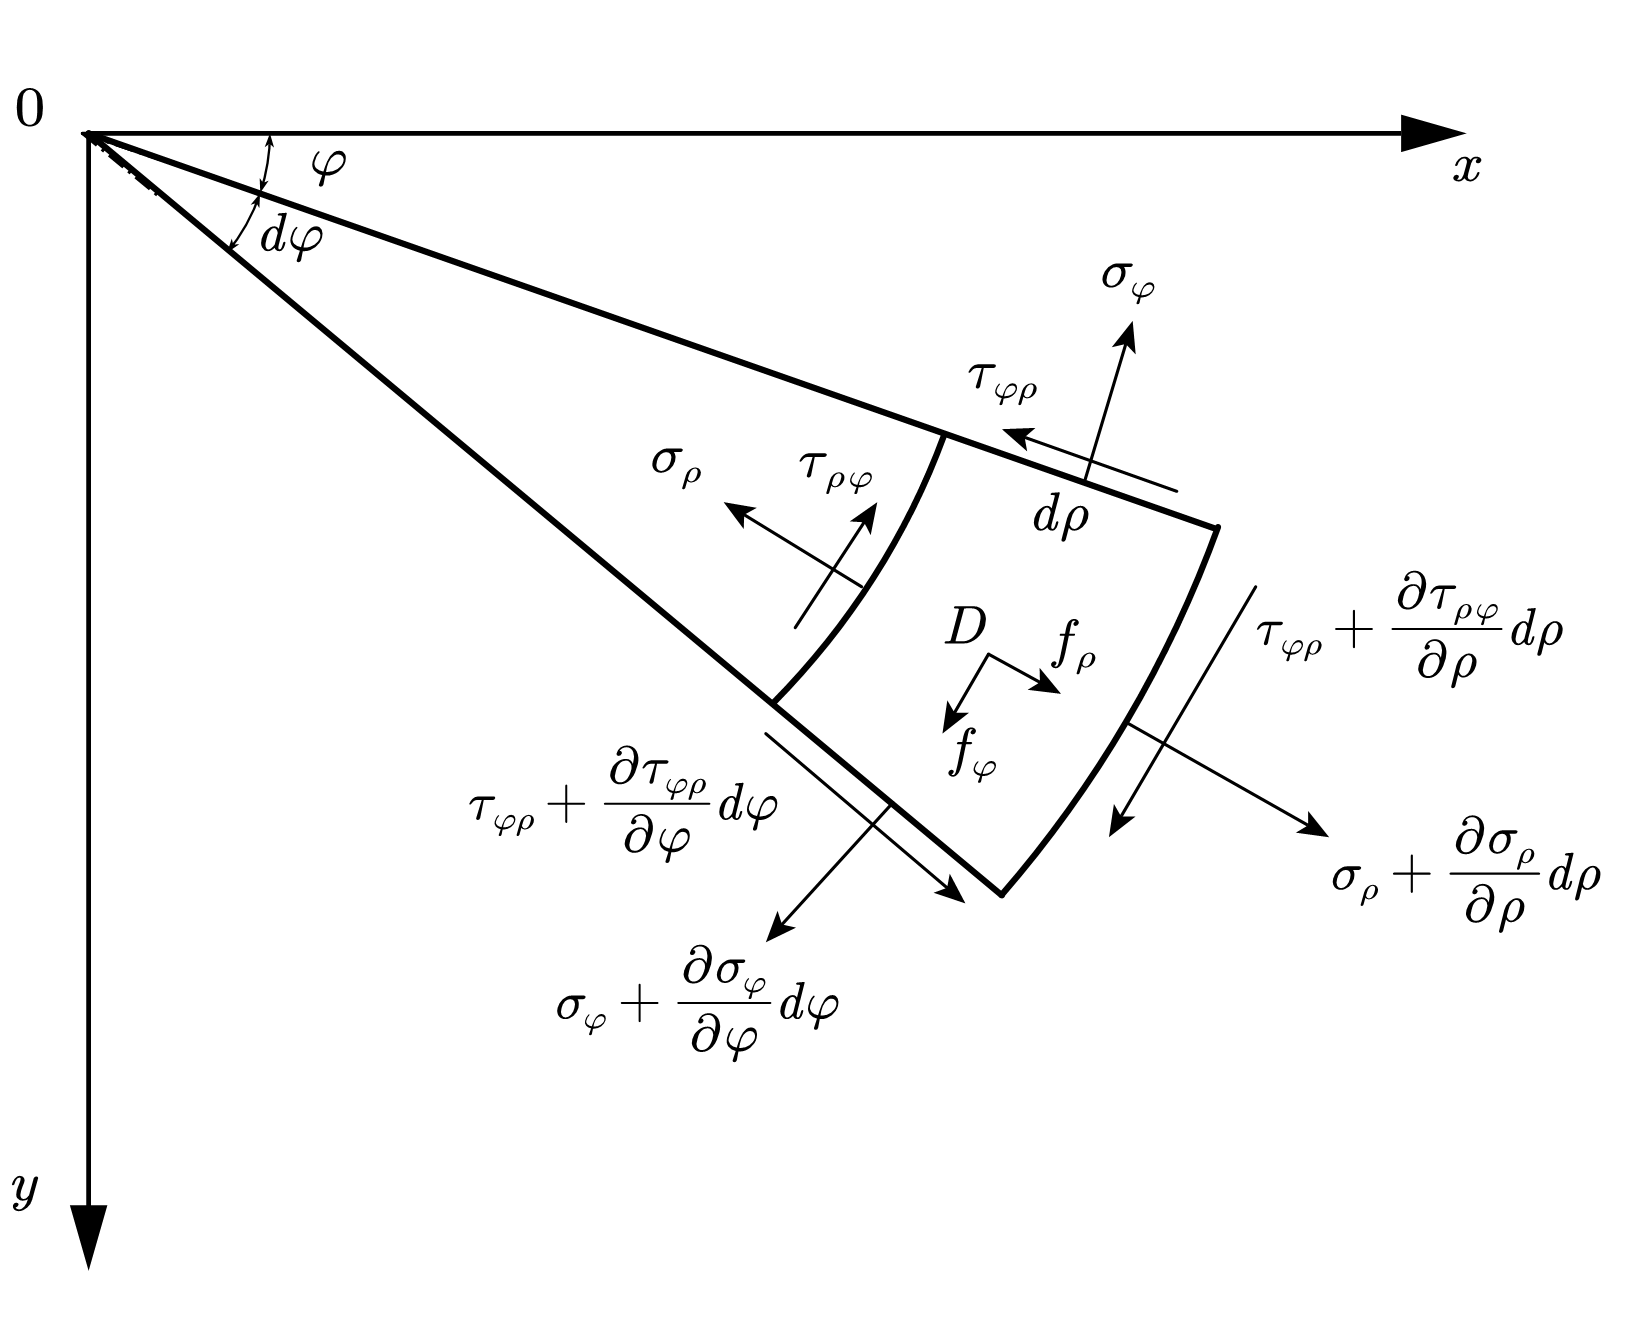
\includegraphics[scale=0.5]{figure/4-1.png}
\caption{}
\end{figure}
\subsubsection{极坐标中的平衡微分方程}
\begin{equation}
\begin{cases}
\frac{\partial \sigma _{\rho}}{\partial \rho}+\frac{1}{\rho}\frac{\partial \tau _{\rho \varphi}}{\partial \varphi}+\frac{\sigma _{\rho}-\sigma _{\varphi}}{\rho}+f_{\rho}=0\\
\frac{1}{\rho}\frac{\partial \sigma _{\varphi}}{\partial \varphi}+\frac{\partial \tau _{\rho \varphi}}{\partial \rho}+\frac{2\tau _{\rho \varphi}}{\rho}+f_{\varphi}=0\\
\end{cases}
\end{equation}

\subsection{极坐标中的几何方程和物理方程}
\subsubsection{极坐标中的几何方程}
\begin{equation}
\begin{cases}
\varepsilon _{\rho}=\frac{\partial u_{\rho}}{\partial \rho}\\
\varepsilon _{\varphi}=\frac{u_{\rho}}{\rho}+\frac{1}{\rho}\frac{\partial u_{\rho}}{\partial \varphi}\\
\gamma _{\rho \varphi}=\frac{1}{\rho}\frac{\partial u_{\rho}}{\partial \varphi}+\frac{\partial u_{\rho}}{\partial \rho}-\frac{u_{\varphi}}{\rho}\\
\end{cases}
\end{equation}
\subsubsection{极坐标中的物理方程}
\begin{equation}
\begin{cases}
\varepsilon _{\rho}=\frac{1}{E}\left( \sigma _{\rho}-\mu \sigma _{\varphi} \right)\\
\varepsilon _{\varphi}=\frac{1}{E}\left( \sigma _{\varphi}-\mu \sigma _{\rho} \right)\\
\gamma _{\rho \varphi}=\frac{1}{G}\tau _{\rho \varphi}=\frac{2\left( 1+\mu \right)}{E}\tau _{\rho \varphi}\\
\end{cases}
\end{equation}
平面应变的情况下,需将上式中的$E$换为$\frac{E}{1-\mu ^2}$,$\mu$换为$\frac{\mu}{1-\mu}$。

\subsection{坐标变换}
\subsubsection{位移分量的坐标变换}
\begin{figure}[!h]
\centering
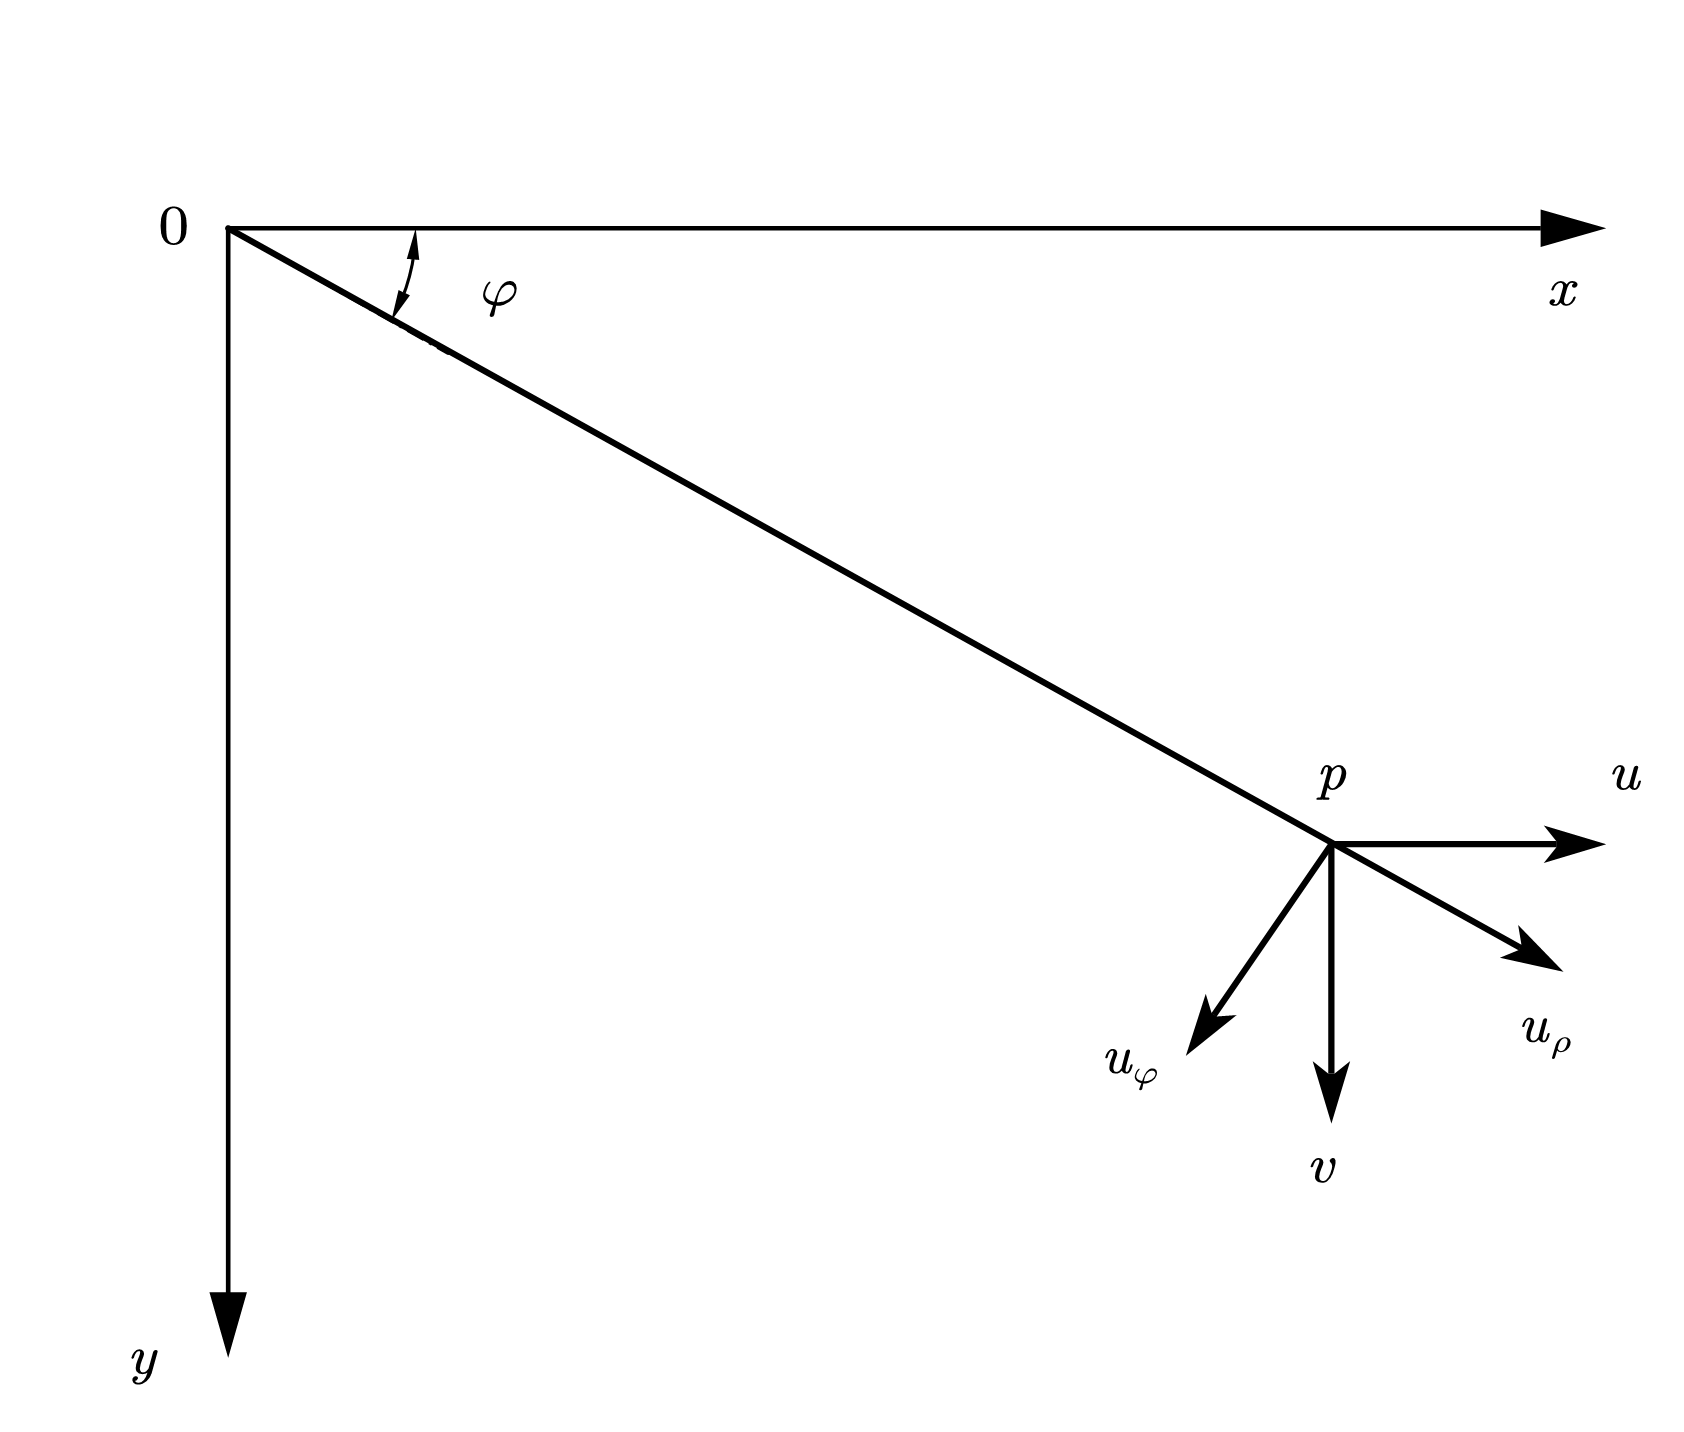
\includegraphics[scale=0.5]{figure/4-2.png}
\caption{}
\end{figure}
\begin{equation}
\begin{cases}
u_{\rho}=u\cos \varphi +v\sin \varphi\\
u_{\varphi}=-u\sin \varphi +v\cos \varphi\\
\end{cases}\Longrightarrow \left( \begin{array}{c}
u_{\rho}\\
u_{\varphi}\\
\end{array} \right) =\left[ \begin{matrix}
\cos \varphi&		\sin \varphi\\
-\sin \varphi&		\cos \varphi\\
\end{matrix} \right] 
,
	\left( \begin{array}{c}
u\\
v\\
\end{array} \right) =\left[ \begin{matrix}
\cos \varphi&		-\sin \varphi\\
\sin \varphi&		\cos \varphi\\
\end{matrix} \right] \left( \begin{array}{c}
u_{\rho}\\
u_{\varphi}\\
\end{array} \right) 
\end{equation}
\subsubsection{应力分量的坐标变换}
\begin{figure}[!h]
\centering
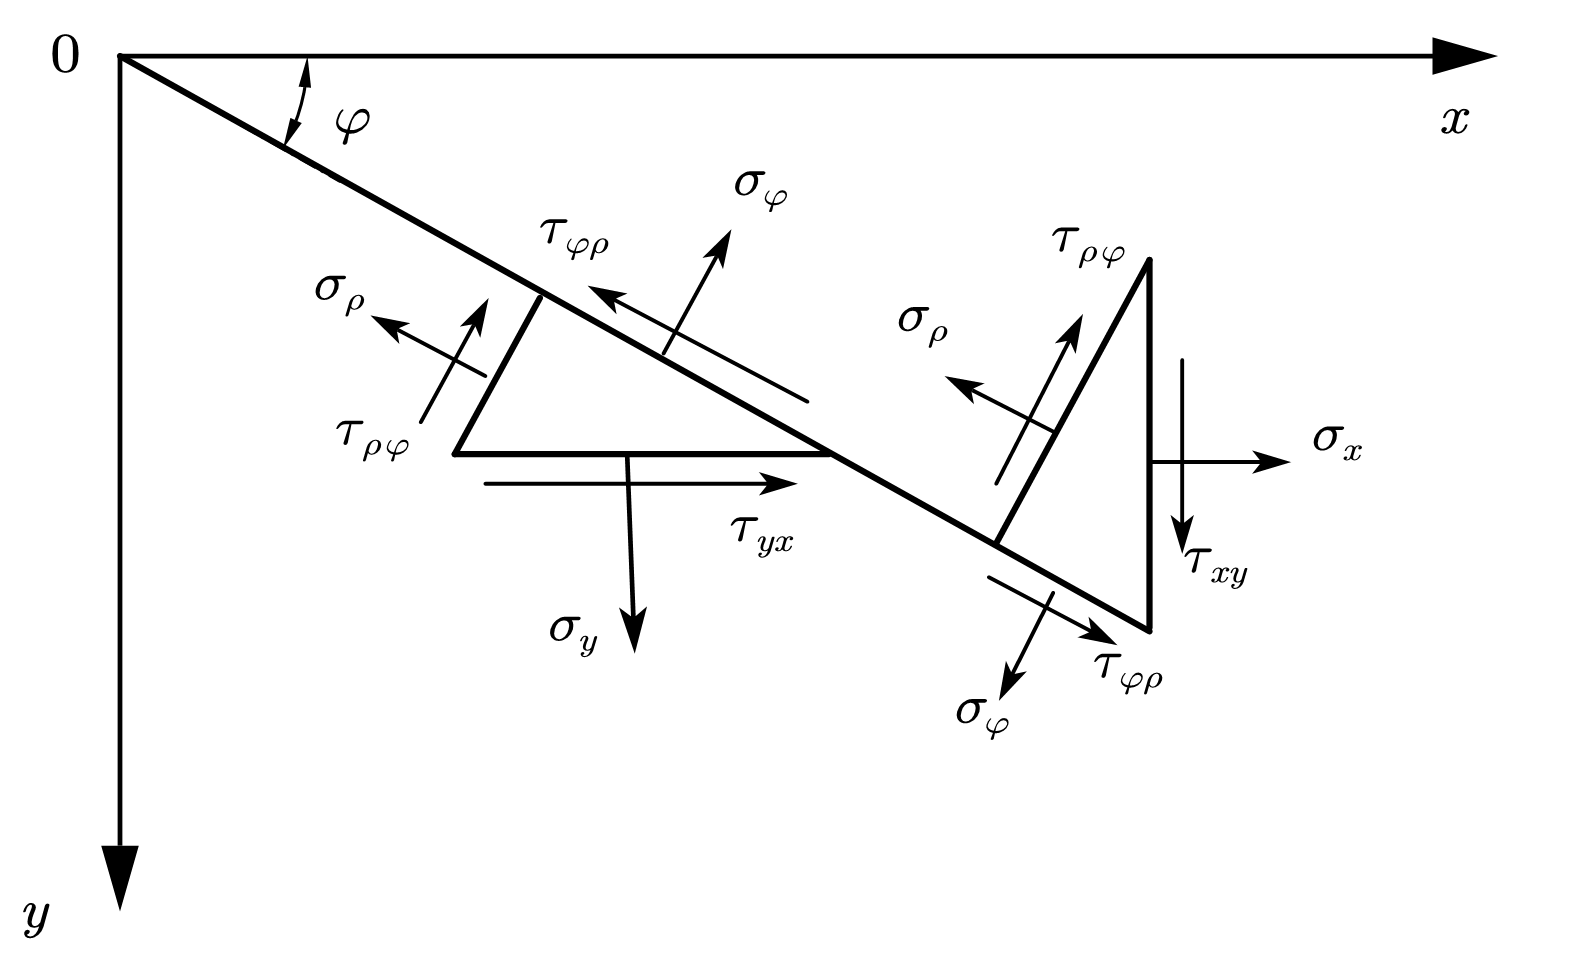
\includegraphics[scale=0.5]{figure/4-3.png}
\caption{}
\end{figure}
\begin{equation}
\begin{cases}
\sigma _x=\sigma _{\rho}\cos ^2\varphi +\sigma _{\varphi}\sin ^2\varphi -2\tau _{\rho \varphi}\sin \varphi \cos \varphi\\
\sigma _y=\sigma _{\rho}\sin ^2\varphi +\sigma _{\varphi}\cos ^2\varphi +2\tau _{\varphi \rho}\sin \varphi \cos \varphi\\
\tau _{xy}=\frac{\sigma _{\rho}-\sigma _{\varphi}}{2}\sin 2\varphi +\tau _{\rho \varphi}\cos 2\varphi\\
\end{cases}
\end{equation}
\begin{equation}
\begin{cases}
\sigma _x=\frac{\sigma _{\rho}+\sigma _{\varphi}}{2}+\frac{\sigma _{\rho}-\sigma _{\varphi}}{2}\cos 2\varphi -\tau _{\rho \varphi}\sin 2\varphi\\
\sigma _y=\frac{\sigma _{\rho}+\sigma _{\varphi}}{2}-\frac{\sigma _{\rho}-\sigma _{\varphi}}{2}\cos 2\varphi -\tau _{\rho \varphi}\sin 2\varphi\\
\tau _{xy}=\frac{\sigma _{\rho}-\sigma _{\varphi}}{2}\sin 2\varphi +\tau _{\rho \varphi}\cos 2\varphi\\
\end{cases}
\\
\end{equation}
\begin{equation}
\left[ \begin{matrix}
\sigma _x&		\tau _{xy}\\
\tau _{yx}&		\sigma _y\\
\end{matrix} \right] =\left[ \begin{matrix}
\cos \varphi&		\sin \varphi\\
-\sin \varphi&		\cos \varphi\\
\end{matrix} \right] \left[ \begin{matrix}
\sigma _{\rho}&		\tau _{\varphi \rho}\\
\tau _{\rho \varphi}&		\sigma _{\varphi}\\
\end{matrix} \right] \left[ \begin{matrix}
\cos \varphi&		\sin \varphi\\
-\sin \varphi&		\cos \varphi\\
\end{matrix} \right] ^T
\end{equation}
\begin{figure}[!h]
	\centering
	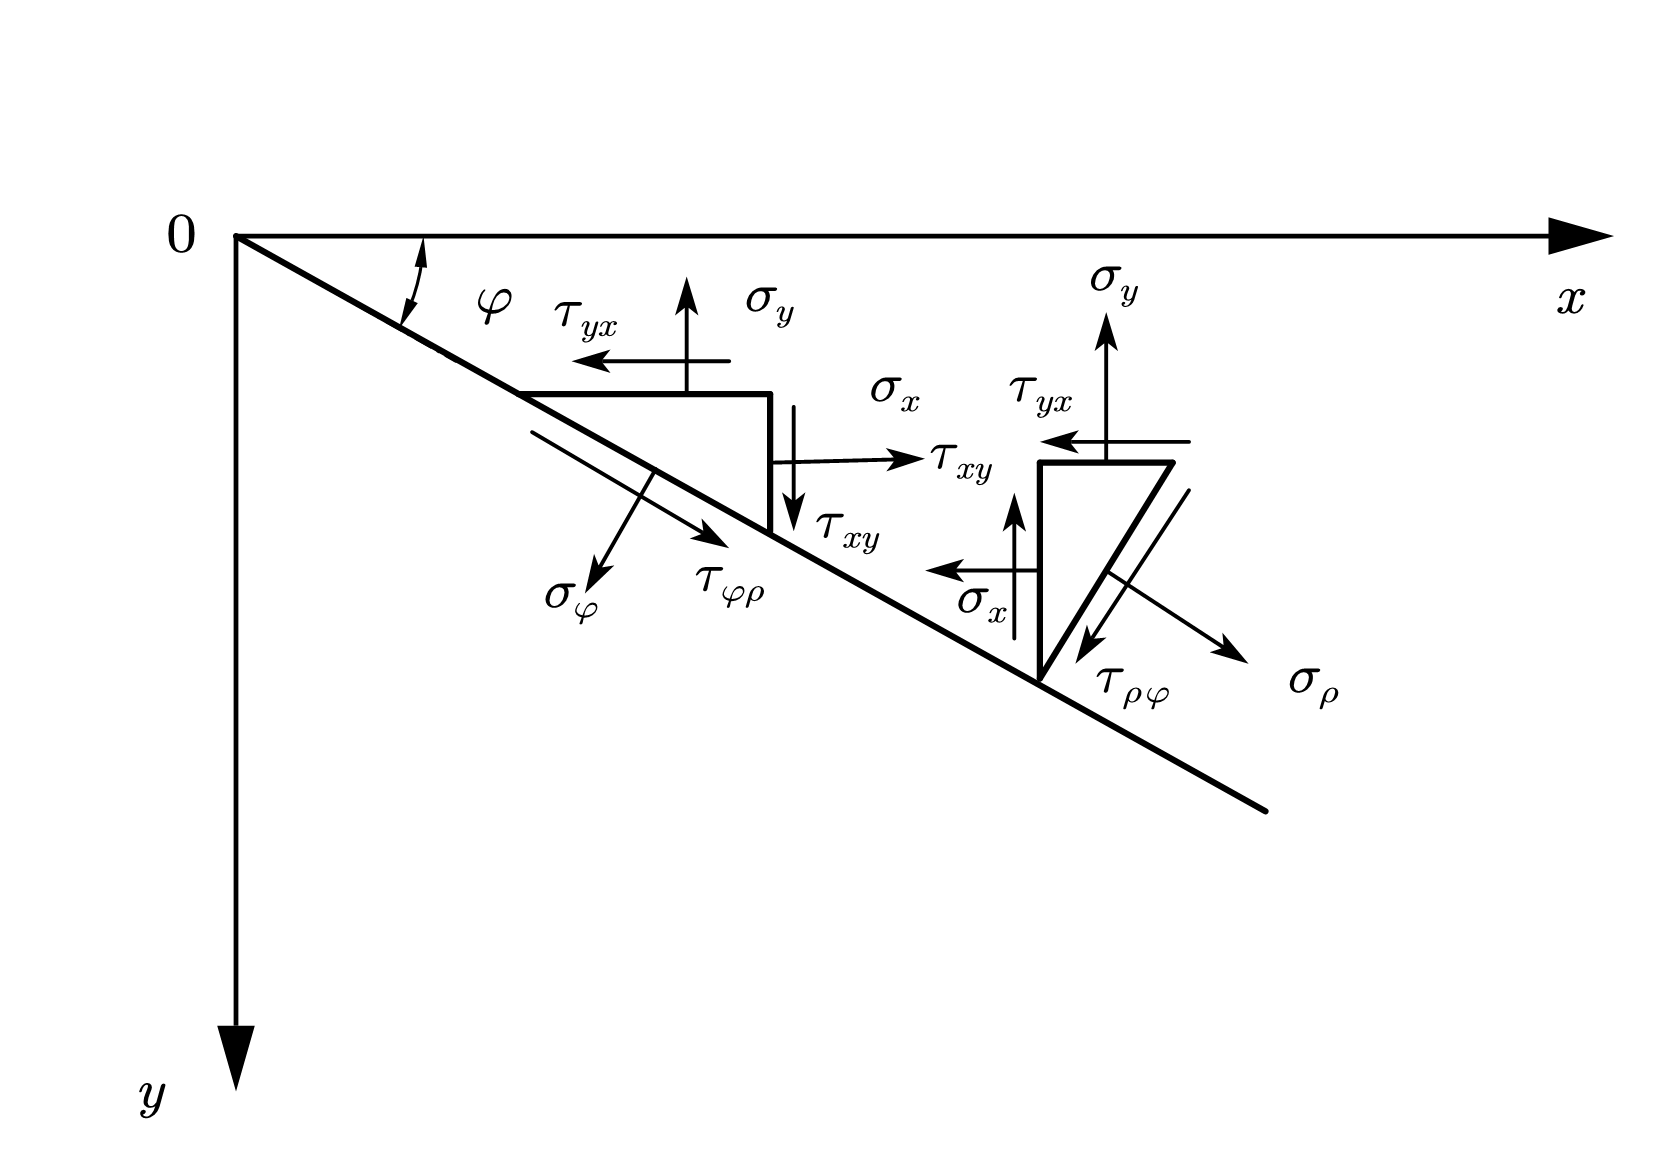
\includegraphics[scale=0.5]{figure/4-4.png}
	\caption{}
\end{figure}
\begin{equation}
\begin{cases}
\sigma _{\rho}=\sigma _x\cos ^2\varphi +\sigma _y\sin ^2\varphi +2\tau _{xy}\sin \varphi \cos \varphi\\
\sigma _{\varphi}=\sigma _x\sin ^2\varphi +\sigma _y\cos ^2\varphi -2\tau _{xy}\sin \varphi \cos \varphi\\
\tau _{\rho \varphi}=\left( \sigma _y-\sigma _x \right) \sin \varphi \cos \varphi +\tau _{xy}\left( \cos ^2\varphi -\sin ^2\varphi \right)\\
\end{cases}
\end{equation}
\begin{equation}
\begin{cases}
\sigma _{\rho}=\frac{\sigma _x+\sigma _y}{2}+\frac{\sigma _x-\sigma _y}{2}\cos 2\varphi +\tau _{xy}\sin 2\varphi\\
\sigma _{\varphi}=\frac{\sigma _x+\sigma _y}{2}-\frac{\sigma _x-\sigma _y}{2}\cos 2\varphi -\tau _{xy}\sin 2\varphi\\
\tau _{\varphi \rho}=\frac{\sigma _x-\sigma _y}{2}\sin 2\varphi +\tau _{xy}\cos 2\varphi\\
\end{cases}
\end{equation}
\begin{equation}
\left[ \begin{matrix}
\sigma _{\rho}&		\tau _{\varphi \rho}\\
\tau _{\rho \varphi}&		\sigma _{\varphi}\\
\end{matrix} \right] =\left[ \begin{matrix}
\cos \varphi&		\sin \varphi\\
-\sin \varphi&		\cos \varphi\\
\end{matrix} \right] ^T\left[ \begin{matrix}
\sigma _x&		\tau _{xy}\\
\tau _{yx}&		\sigma _y\\
\end{matrix} \right] \left[ \begin{matrix}
\cos \varphi&		\sin \varphi\\
-\sin \varphi&		\cos \varphi\\
\end{matrix} \right]
\end{equation}
\subsection{极坐标中的应力函数与相容方程}
当$f_{\rho}=f_{\varphi}=0$时:
\begin{equation}\begin{cases}
\sigma _{\rho}=\frac{1}{\rho}\frac{\partial \varPhi}{\partial \rho}+\frac{1}{\rho ^2}\frac{\partial ^2\varPhi}{\partial \varphi ^2}\\
\sigma _{\varphi}=\frac{\partial ^2\varPhi}{\partial \rho ^2}\\
\tau _{\rho \varphi}=-\frac{\partial}{\partial \rho}\left( \frac{1}{\rho}\frac{\partial \varPhi}{\partial \varphi} \right)\\
\end{cases}
\\
\end{equation}
\subsubsection{相容方程}
\begin{equation}
\left( \frac{\partial ^2}{\partial \rho ^2}+\frac{1}{\rho}\frac{\partial}{\partial \rho}+\frac{1}{\rho ^2}\frac{\partial ^2}{\partial \varphi ^2} \right)^2 \varPhi =0
\end{equation}
\subsection{轴对称应力和相容的位移}
所谓轴对称问题,是指物体几何形状或某物理量是绕某一轴对称的,凡通过此轴的任何面均为对称面。如果该物体所受外部荷载也对称于该轴,那么相应所产生的应力也必对称该轴。
\\
令$\varPhi =\varPhi \left( \rho \right) $
\begin{equation}
\sigma _{\rho}=\frac{1}{\rho}\frac{d\varPhi}{d\rho}\,\,,     \sigma _{\varphi}=\frac{d^2\varPhi}{d\rho ^2},     \tau _{\rho \varphi}=0
\end{equation}
\begin{equation}
\left( \frac{\partial ^2}{\partial \rho ^2}+\frac{1}{\rho}\frac{\partial}{\partial \rho} \right) \varPhi =0
\end{equation}
即
\begin{equation}
\varPhi =A\ln \rho +B\rho ^2\ln \rho +C\rho ^2+D
\end{equation}
应力分量
\begin{equation}
\begin{cases}
\sigma _{\rho}=\frac{A}{\rho ^2}+B\left( 1+2\ln \rho \right) +2C\\
\sigma _{\varphi}=-\frac{A}{\rho ^2}+B\left( 3+2+\ln \rho \right) +2C\\
\tau _{\rho \varphi}=0\\
\end{cases}
\end{equation}
代入物理方程和几何方程可得位移分量
\begin{equation}
\begin{cases}
u_{\rho}=\frac{1}{E}\left[ -\left( 1+\mu \right) \frac{A}{\rho}+2\left( 1-\mu \right) B\rho \left( \ln \rho -1 \right) +\left( 1-3\mu \right) B\rho +2\left( 1-\mu \right) C\rho \right] +I\cos \varphi +K\sin \varphi\\
u_{\varphi}=\frac{4B\rho \varphi}{E}+H\rho -I\sin \varphi +K\cos \varphi\\
\end{cases}
\end{equation}
\begin{enumerate}
\item 在轴对称应力条件下,应力、应变和位移的通解,适用于任何轴对称应力问题。
\item 在轴对称应力条件下,应变也是轴对称的,但位移不一定是轴对称的。
\item 实现轴对称应力的条件是:物体形状、体力和面力应是轴对称的。
\item 轴对称应力及对应的位移的通解已满足相容方程,它们还需满足边界条件及多连体中的位移单值条件,并由此求出系数A、B、C。
\end{enumerate}
\begin{note}
欧拉方程:
\[x^ny^{\left( n \right)}+P_1x^{n-1}y^{\left( n-1 \right)}+\cdots +P_{n-1}xy'+P_ny=0\]
特征方程为:
\[\left[ k\left( k-1 \right) \cdots \left( k-n+1 \right) +P_1\left[ k\left( k-1 \right) \cdots \left( k-n+2 \right) \right] +\cdots +P_{n-1}k+P_n \right] =0\]
关于$K$的$n$次代数方程,可解得n个特征根$k_1\text{、}k_2\text{、}\cdots k_n$
\begin{enumerate}
\item 当它们是互不相等的实根时,通解具有幂函数的形式
\[y=C_1x^{k_1}+C_2x^{k_2}+\cdots +C_nx^{k_n}\]
\item 每当出现重根时,每多一重根,就多乘一个$\ln x$\\
如:当$k_1$为$m\left( m<n \right) $重根时,通解为
\[y=C_1x^{k_1}+C_2x^{k_2}\ln x+\cdots +C_mx^{k_1}\ln ^{m-1}x+C_{m+1}x^{k_{m+1}}+\cdots +C_nx^{k_n}\]
\item 出现共轭复根时,则虚部是三角函数因子\\
如: 当$k_{1,2}=\alpha \pm i\beta $,通解为
\[y=C_1x^{\alpha}\cos \left( \beta \ln x \right) +C_2x^{\alpha}\sin \left( \beta \ln x \right) +C_3x^{k_3}+\cdots +C_nx^{k_n}\]
\item 当出现复重根,则实部要多乘因子$\ln x$\\
如:$k_{1,2}=\alpha \pm i\beta $为$m\left( m<\frac{n}{2} \right) $重共轭复根时,通解为
\begin{align*}
	y
	= & \left[ C_1x^{\alpha}+C_2x^{\alpha}\ln x+\cdots +C_mx^{\alpha}\ln ^{m-1}x \right] \cos \left( \beta \ln x \right) +\\
	&\left[ C_{m+1}x^{\alpha}+C_{m+2}x^{\alpha}\ln x+\cdots +C_{2m}x^{\alpha}\ln ^{m-1}x \right] \sin \left( \beta \ln x \right) +\\
	&C_{2m+1}x^{k_{2m+1}}+\cdots +C_nx^{k_n}
\end{align*}
\end{enumerate}
\end{note}

\begin{example}
试求解平面轴对称应力问题的相容方程\[\rho ^4\varPhi ^{\left( 4 \right)}+2\rho ^3\varPhi ^{\left( 3 \right)}-\rho ^2\varPhi ''+\rho \varPhi '=0\]
\end{example}
	\begin{remark}
	特征方程:
	\[k\left( k-1 \right) \left( k-2 \right) \left( k-3 \right) +2k\left( k-1 \right) \left( k-2 \right) -k\left( k-1 \right) +k=0\]
	解得:$$k_{1,2}=0,k_{3,4}=2$$\\
	得:$$\varPhi =A\ln \rho +B\rho ^2\ln \rho +C\rho ^2+D$$
	\end{remark}

\begin{example}
试求解如下的常微分方程
\[\rho ^4f^{\left( 4 \right)}\left( \rho \right) +2\rho ^3f'''\left( \rho \right) -9\rho ^2f''\left( \rho \right) +9\rho f'\left( \rho \right) =0\]
\end{example}
	\begin{remark}
		特征方程:
		\[k\left( k-1 \right) \left( k-2 \right) \left( k-3 \right) +2k\left( k-1 \right) \left( k-2 \right) -9k\left( k-1 \right) +9k=0\]
		解得:\[k_1=4,k_2=2,k_3=0,k_4=-2\]
		得:\[\]
	\end{remark}
